\documentclass{article}

% if you need to pass options to natbib, use, e.g.:
%     \PassOptionsToPackage{numbers, compress}{natbib}
% before loading neurips_2020

% ready for submission
% \usepackage{neurips_2020}

% to compile a preprint version, e.g., for submission to arXiv, add add the
% [preprint] option:
%     \usepackage[preprint]{neurips_2020}

% to compile a camera-ready version, add the [final] option, e.g.:
     \usepackage[final]{Lorenzo_Tibaldi_Arezou_Ranjbarpour_Maralani_Report}

% to avoid loading the natbib package, add option nonatbib:
%     \usepackage[nonatbib]{neurips_2020}

\usepackage[utf8]{inputenc} % allow utf-8 input
\usepackage[T1]{fontenc}    % use 8-bit T1 fonts
\usepackage{hyperref}       % hyperlinks
\usepackage{url}            % simple URL typesetting
\usepackage{booktabs}       % professional-quality tables
\usepackage{amsfonts}       % blackboard math symbols
\usepackage{nicefrac}       % compact symbols for 1/2, etc.
\usepackage{microtype}      % microtypography


\usepackage{graphicx}

\title{Speaker Recognition Report}
\author{
	Lorenzo Tibaldi\\
	\texttt{s4347466@studenti.unige.it}
	\AND 
	Arezou Ranjbarpour Maralani\\
  	\texttt{s4847076@studenti.unige.it}}
	
	
\begin{document}

\maketitle
\begin{abstract}
Speaker Recognition is the problem of using some ad hoc features 
to be able to recognize the speaker of a new audio sample from a database of known speakers.
In this project we tackled the problem by implementing a small neural network model.
\end{abstract}

\section{Introduction}
	\subsection{The code}
	The python code we wrote for the project can be found at: \url{https://github.com/WeLikeIke/SpeakerRecognition_Project}.\label{url:repo}

	The code was tested completely on Google Collaboratory and was developed using the keras library for neural networks.

	\subsection{The dataset}
	The dataset is called SoundData.zip and can be found in the repository here \ref{url:repo}.

	We decided to create our own dataset instead of downloading one from the internet, for that purpose we used a free recording software: Audacity.

	The dataset is composed of 99 audio files in wav format.
	\begin{itemize}
	\item 33 files from speaker 0 (Lorenzo)
	\item 33 files from speaker 1 (Arezou)
	\item 33 files full of noise
	\end{itemize}
	We included the noise part of the dataset so that the problem wouldn't just be a binary classification problem.

	\subsection{The main challenges}
	The 2 main challenges of this project were:
	\begin{enumerate}
	\item Finding a satisfactory balance between a small dataset and an accurate model.
	\item Fine tuning the parameters for a while to obtain a pretty good model.
	\end{enumerate}

\section{Implementation}
	\subsection{Choosing the features}
	There are many ways to implement a Speaker Recognition model depending on your needs, 
	we decided to use Mel-frequency cepstral coefficents, or MFCC for short, as the only features our model would take as inputs.

	\subsection{A bit of preprocessing}
	Since it wasn't possible to record meaninful voicelines while adhering to strict timing rules we decided to record many voicelines of different lengths.
	
	Because of that we had to do a small amount of preprocessing, after the extraction of the MFCC we took the longest voiceline (around 15 second) 
	and padded all the other MFCC to the length of that one. \ref{fig:mfcc}

	\begin{figure}
	\centering
	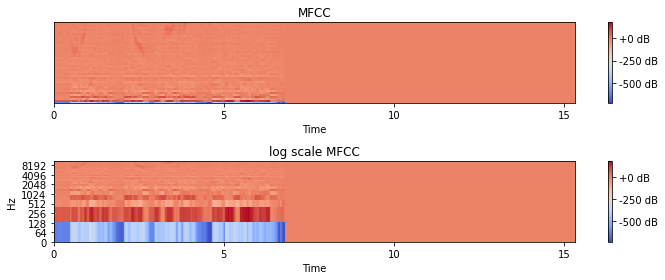
\includegraphics[width = \textwidth]{mfcc}
	\caption{One input of the model, all the MFCC of a single voiceline where the padding on the right is clearly visible.}
	\label{fig:mfcc}
	\end{figure}

	\subsection{Creating the model}
	The model is composed of:
	\begin{itemize}
	\item A Long Short-Term Memory layer with 256 neurons, LSTM are especially useful when the dataset is small (like in our case).
	\item A Flatten layer that needs to be there to go from the output of the LSTM to the input of the Dense layer.
	\item A Dense layer with 128 neurons and ReLU activation function.
	\item Lastly a Dense layer with as many neurons as the possible labels (here 3) with a {\bf softmax} activation function.
	\end{itemize}

\section{Improvements}
	To avoid overfitting we added 2 Dropout layers, one after the LSTM and one after the first Dense layer.

	Then as best practice we added a BatchNormalization layer between the Dense layer and the last Dropout layer.

	Then we turned our attention towards tuning a couple of parameters, we empirically settled on 16 as batch size, 32 as number of epochs, 
	0.5 as the dropout values for the Dropout layers and finally the number of MFCC for each audio file (so the number of inputs for the model) at 40.

	Lastly we were still noticing a bit of overfitting, and we were able to contrast that by adding a dropout value inside the LSTM, recurrent layers like this are
	fairly susceptible to overfitting so we introduced an internal dropout of 0.33.

	Final model architecture here \ref{fig:model}.

	\subsection{A quick tangent}
	As we were recording the voicelines one of the speakers was constantly recording shorter voicelines, we theorized that since we were padding all the 
	MFFC then it could be possible that the model would start to recognize the speaker based on how many zeros were at the end of a feature.

	We didn't want to risk this meta learning behaviour to worsen the model so the next recording session 
	we alternated between long and short voicelines for both speakers. 

\section{Results}
	The model got trained on 64\% of the dataset, validated using 16\% of it and then tested on the last 20\%.

	The final result is a model that performed with an accuracy of around 80\%. \ref{fig:acc}

	Obviously ,since the dataset is small, there can be quite a variation in final accuracies, still 
	the vast majority of times the model returned an accurate prediction for over 60\% of the test set.

	\bigskip
	We are satisfied with this final result, in the future it could surely be possible to improve upon this model, for example by increasing 
	the complexity of the model or introducing different features.

	In particular, if we ignore the noise part of the dataset then it could've been theoretically possible to build a recognition neural network that only uses the
	highest and lowest frequencies in the voicelines, this is because the 2 speakers are one male and one female and as such should have different frequency
	ranges.

	\begin{figure}
	\centering
	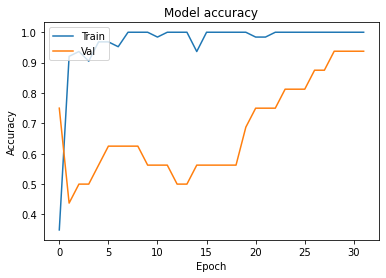
\includegraphics[width = \textwidth]{acc}
	\caption{An example of an accuracy plot during the 32 training epochs.}
	\label{fig:acc}
	\end{figure}

	\begin{figure}
	\centering
	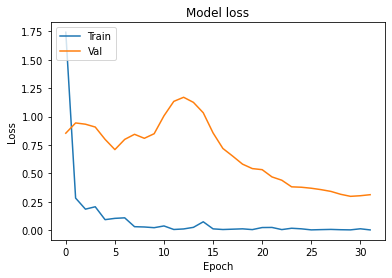
\includegraphics[width = \textwidth]{loss}
	\caption{An example of a loss plot during the 32 training epochs. Of note the peak around the 12th epoch where an early stopping procedure would've 
		     surely blocked the model since the loss was increasing since epoch 6, but then the model recovered and improved quite a bit in the last epochs.}
	\end{figure}

	\begin{figure}
	\centering
	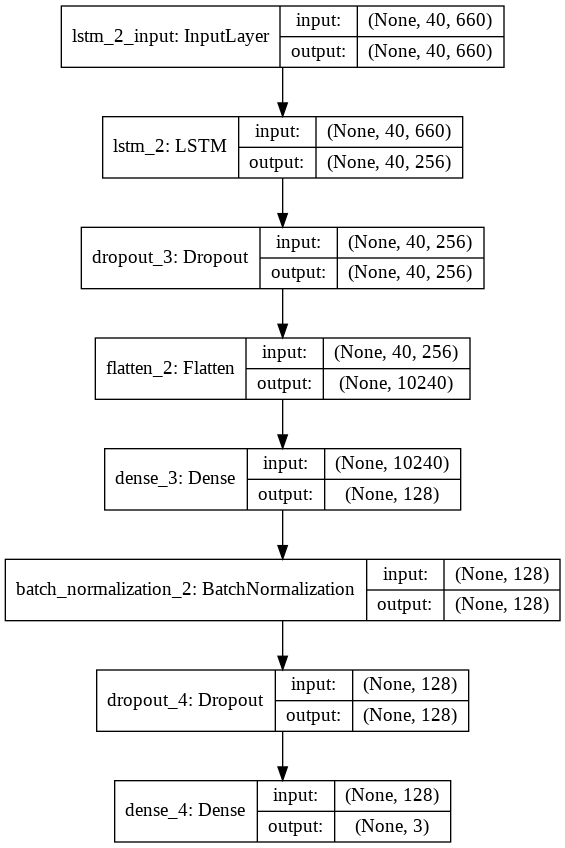
\includegraphics[width = \textwidth]{model}
	\caption{The final version of the model.}
	\label{fig:model}
	\end{figure}

\clearpage
\section*{References}
\begin{enumerate}
\item \url{https://www.researchgate.net/publication/221912826_Speaker_Recognition}
\item \url{https://www.researchgate.net/publication/3333308_Speaker_Recognition_Using_Neural_Networks_And_Conventional_Classifiers}
\item \url{https://www.researchgate.net/publication/313587260_Speech_enhancement_using_Long_Short-Term_Memory_based_recurrent_Neural_Networks_for_noise_robust_Speaker_Verification}
\end{enumerate}
\end{document}
